\chapter{Umsetzung und Ergebnisse}
\label{cha:umsetzung}

Je nach Art der Arbeit kann diese Kapitelüberschrift auch \glqq Ergebnisse\grqq~lauten, z.~B. bei rein messtechnischen Aufgaben.

Beschreibung der Umsetzung des zuvor gewählten Vorgehens (theoretische Untersuchung, Erhebungen, Durchführung von Experimenten, Prototypenaufbau, Implementierung eines Prozesses, etc.).

Verifikation anhand der zuvor erarbeiteten Anforderungen und Validierung in Bezug auf das zuvor gestellte Ziel. Diskussion der Ergebnisse. Spätestens hier auch auf die Zuverlässigkeit der gewonnenen Erkenntnisse eingehen (z.~B. anhand der Genauigkeit von Messergebnissen).

% Linke Hälfte der A3-Seite
%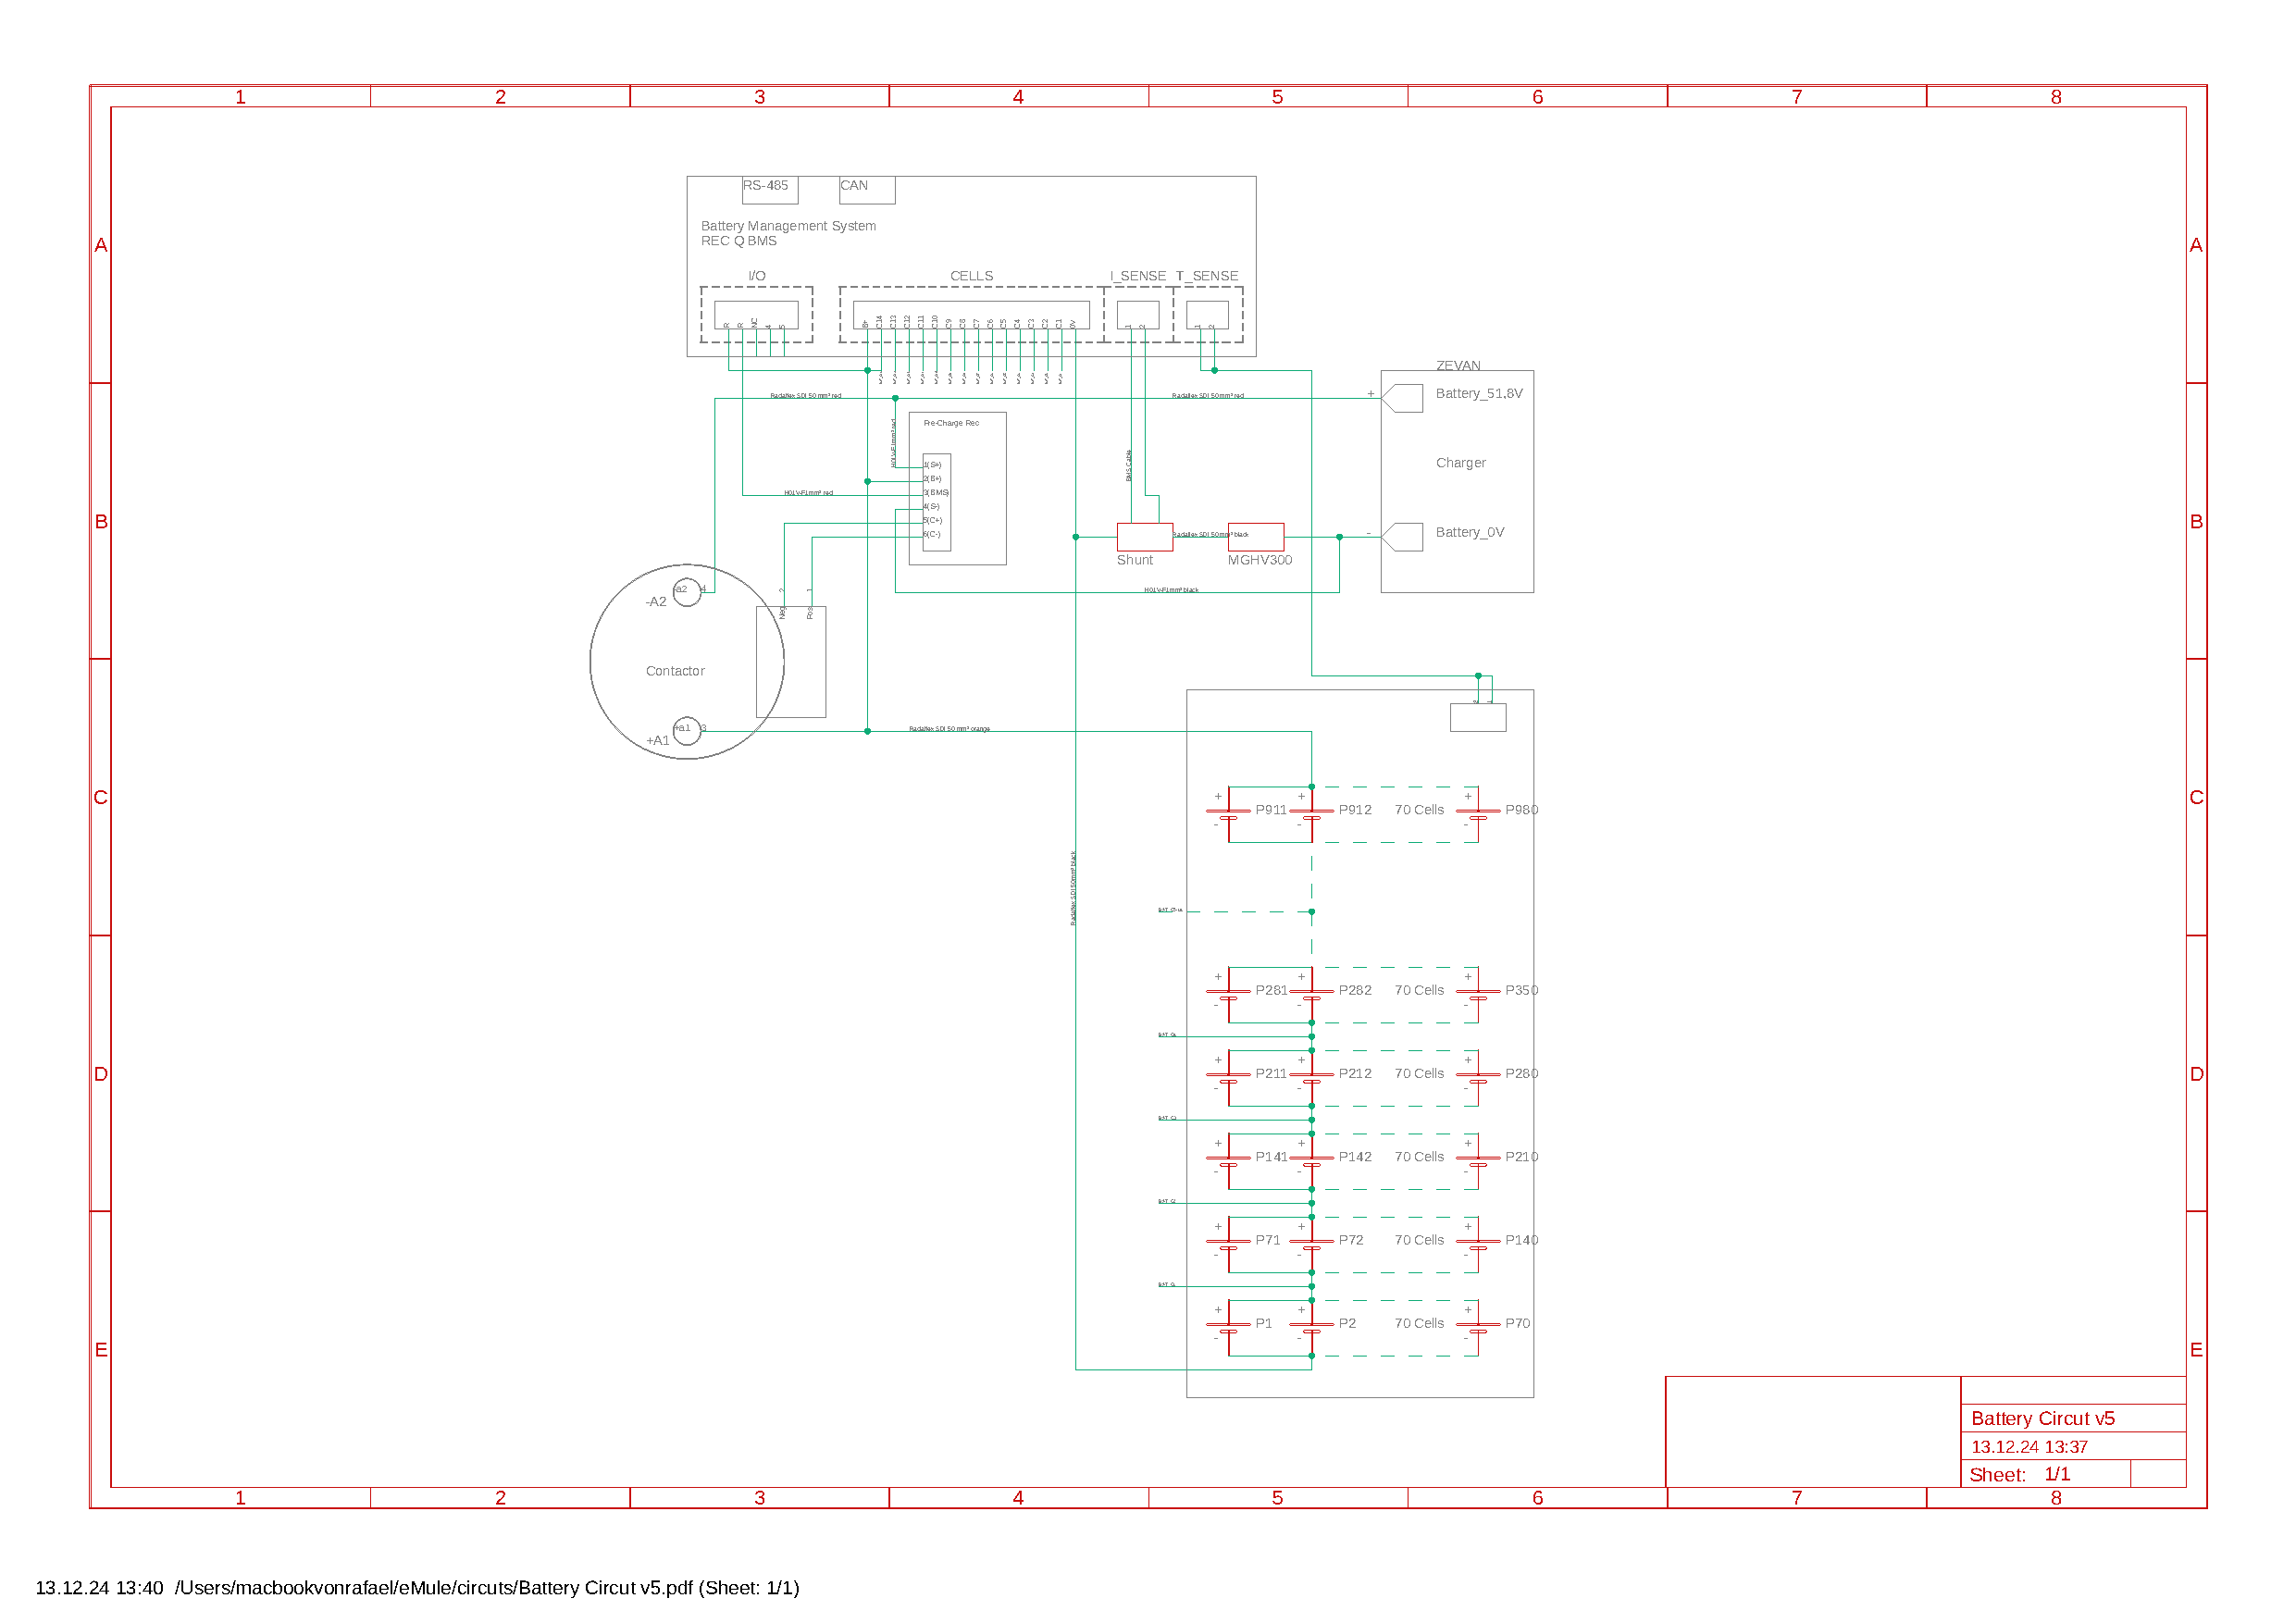
\includepdf[pages=1, trim=0cm 0cm 21cm 0cm, clip]{circuts/Battery Circut v5.pdf}

% Rechte Hälfte der A3-Seite
%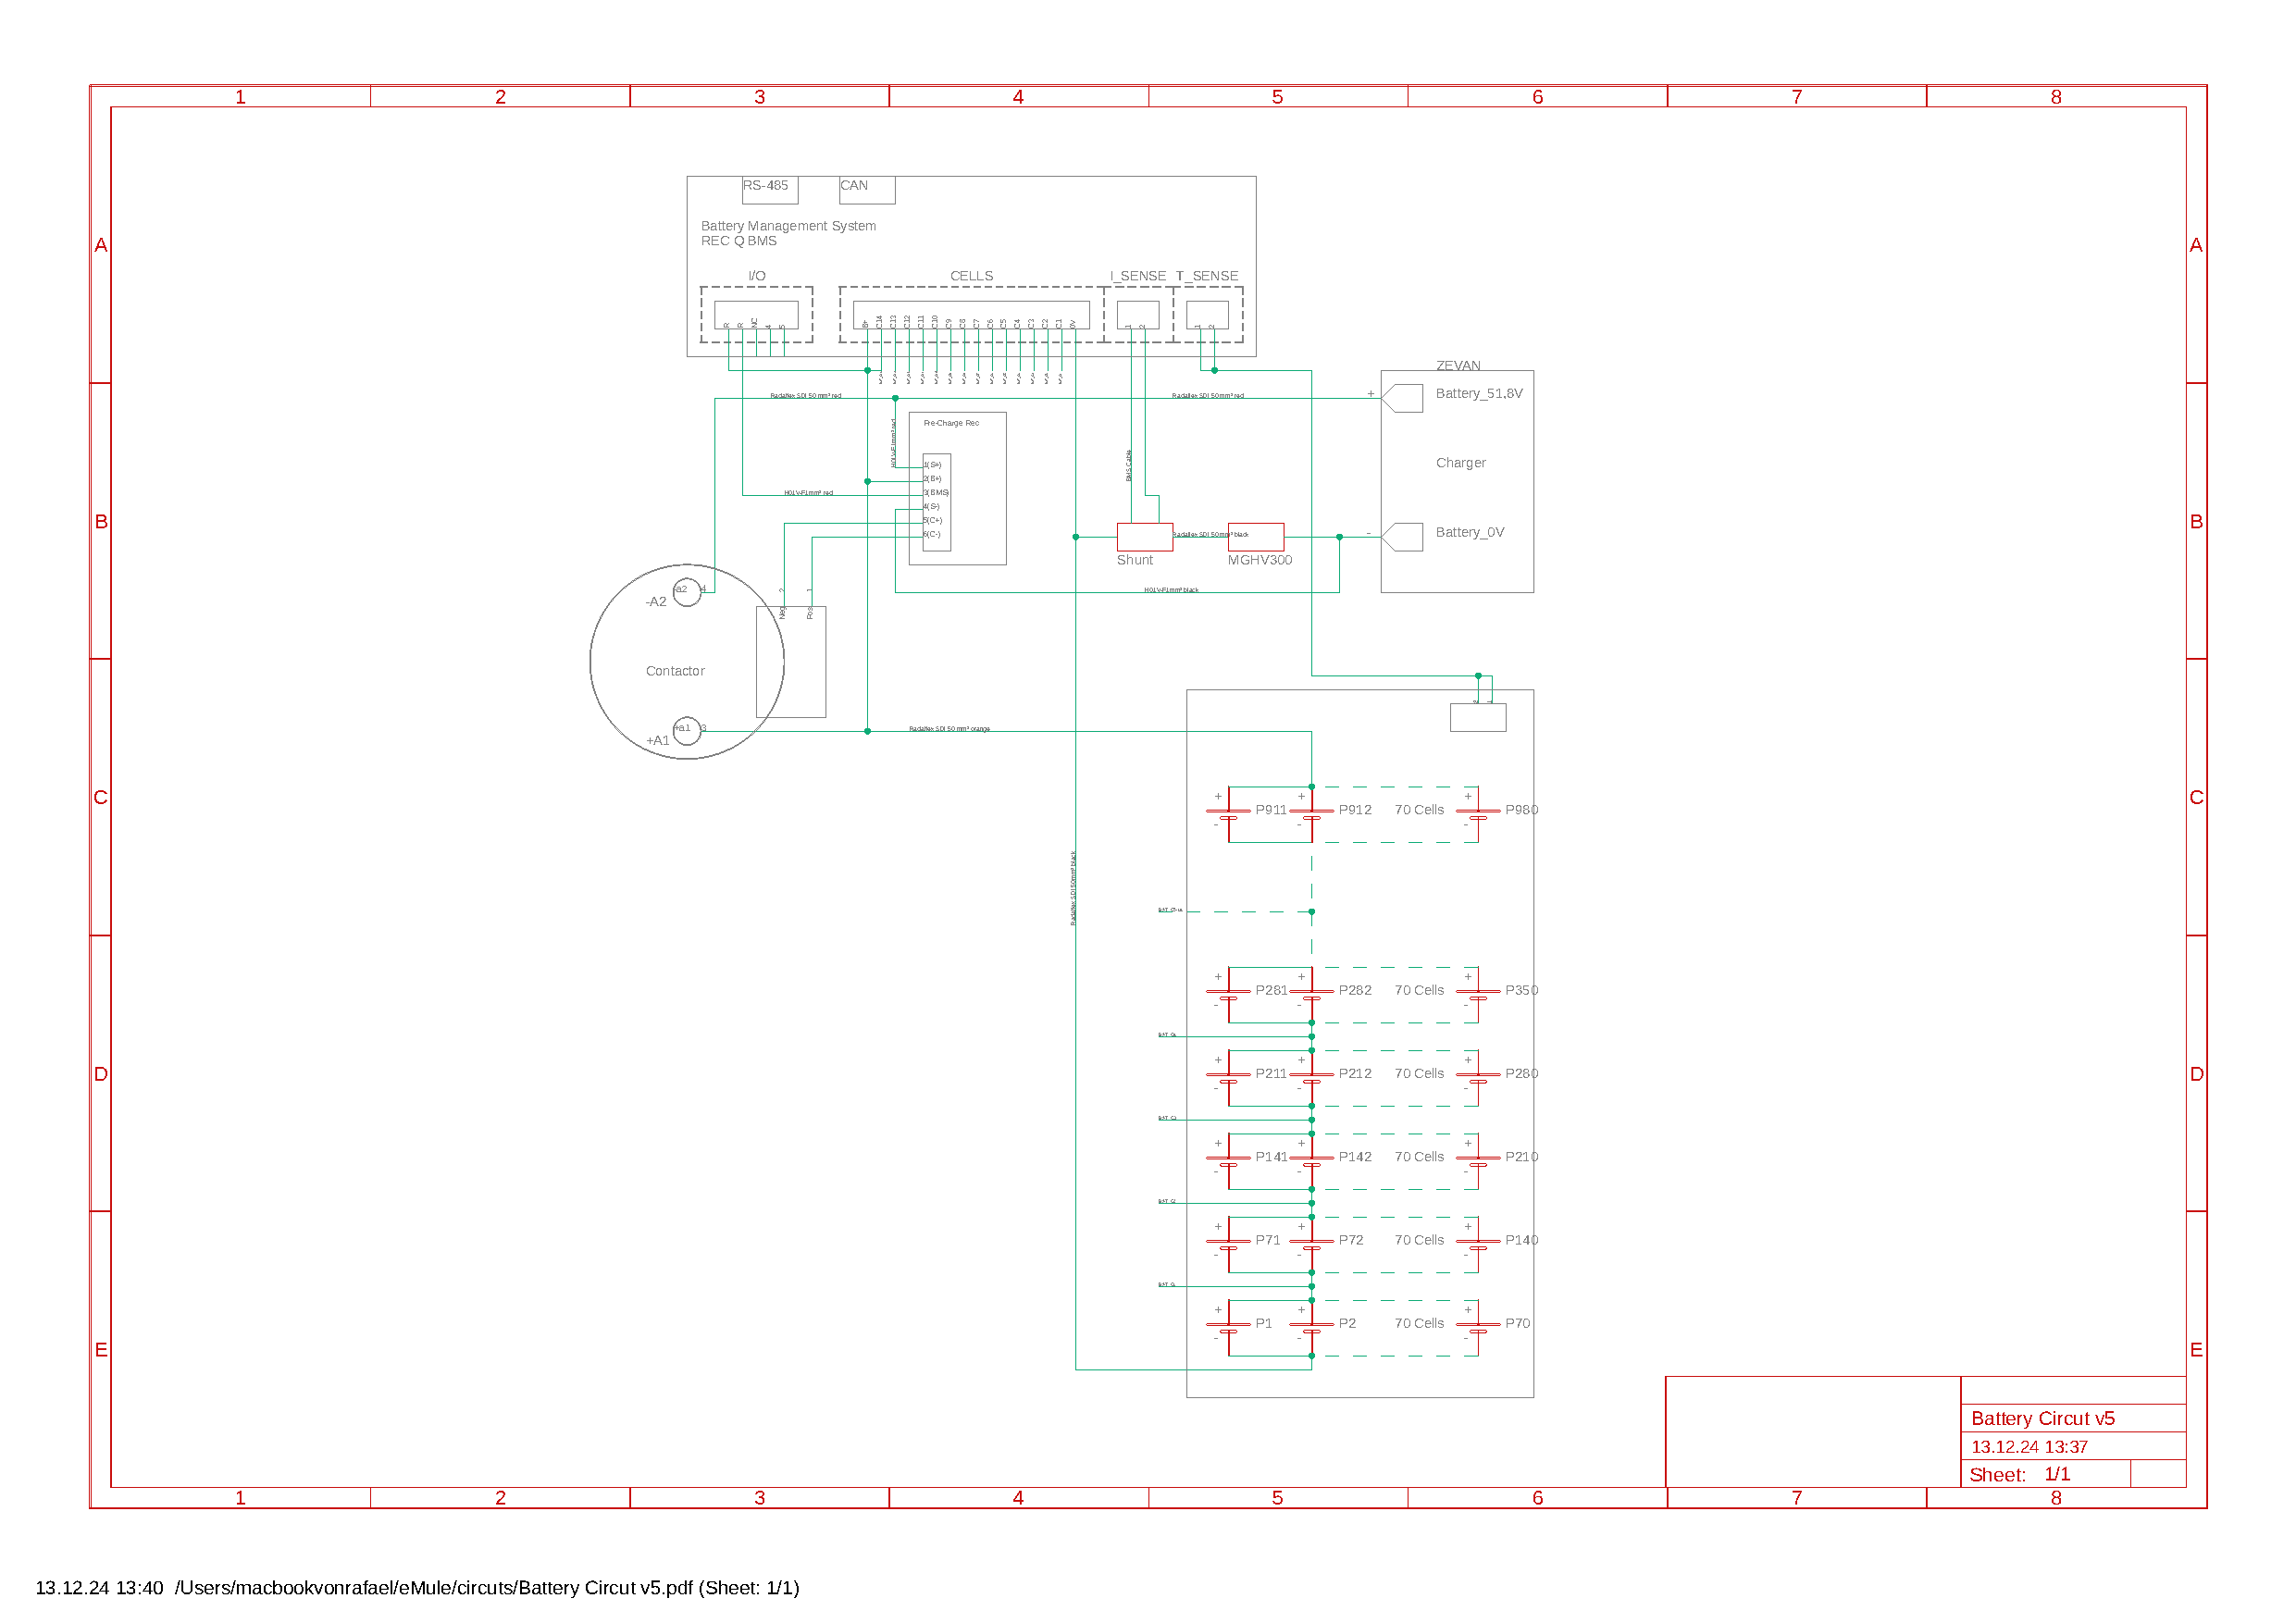
\includepdf[pages=1, trim=21cm 0cm 0cm 0cm, clip]{circuts/Battery Circut v5.pdf}

%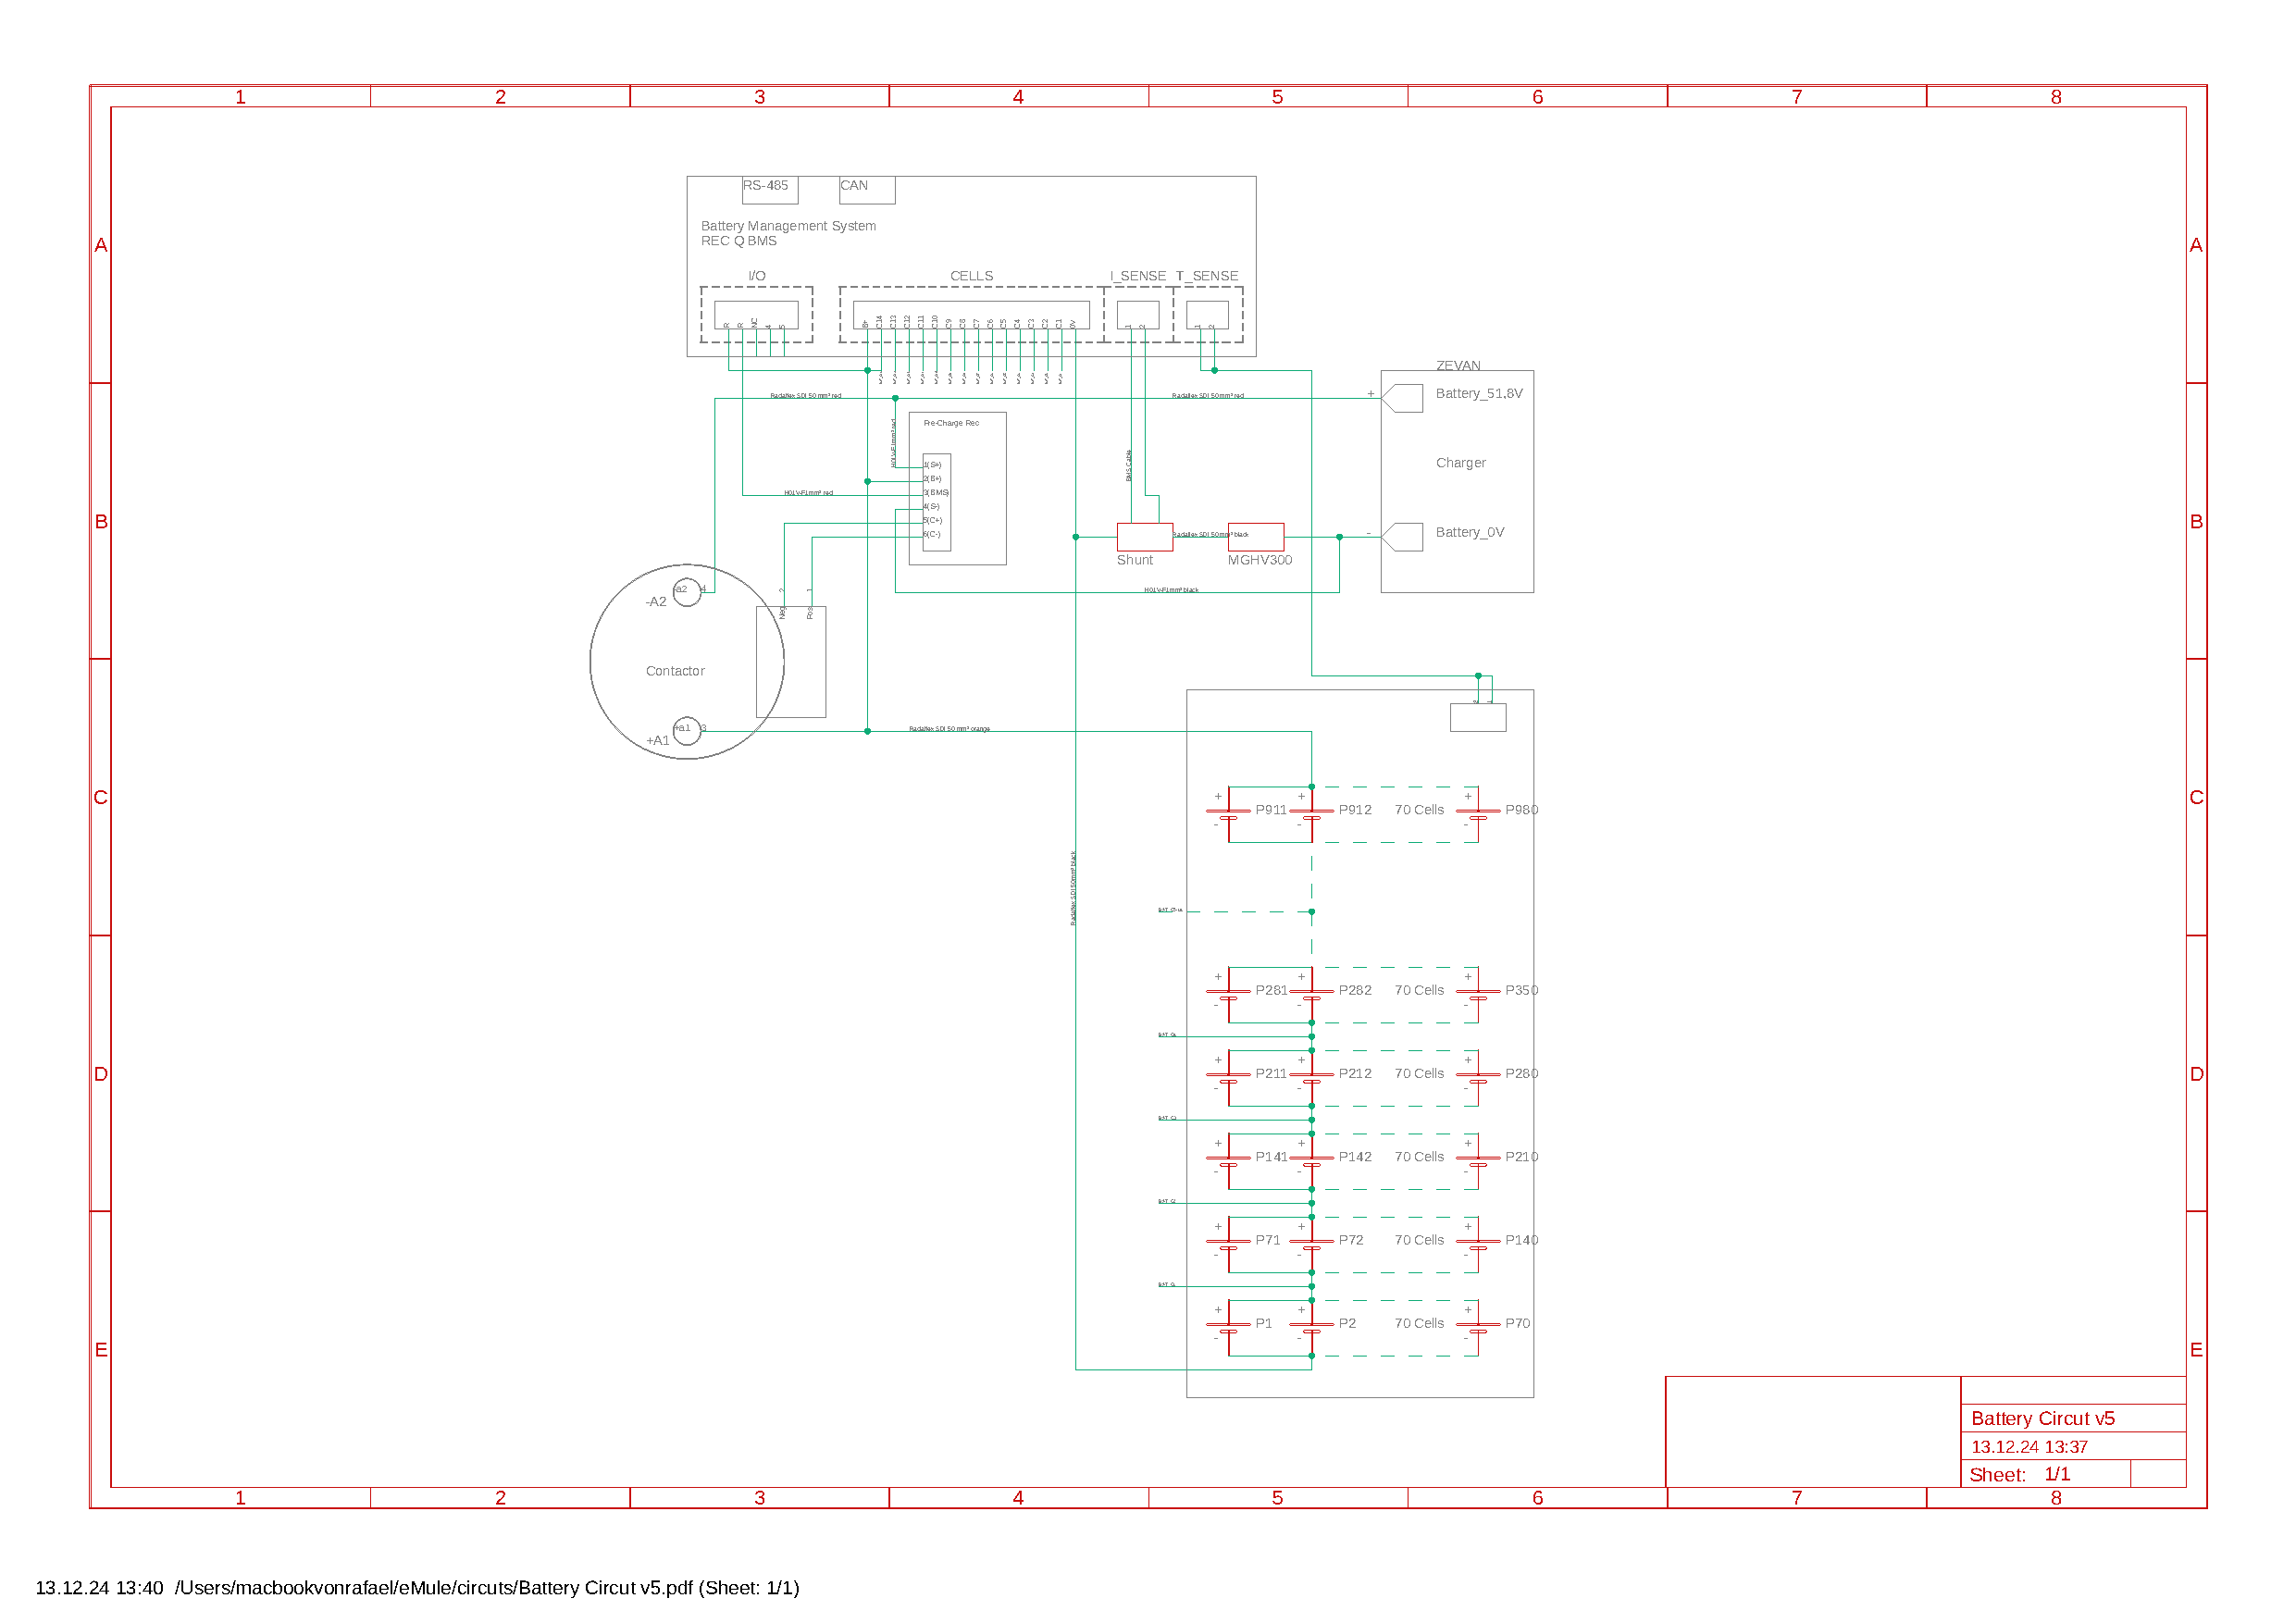
\includepdf[pages=1, angle=90, fitpaper=true]{circuts/Battery Circut v5.pdf}

\section*{Schaltplan Batterie Circuit v5}
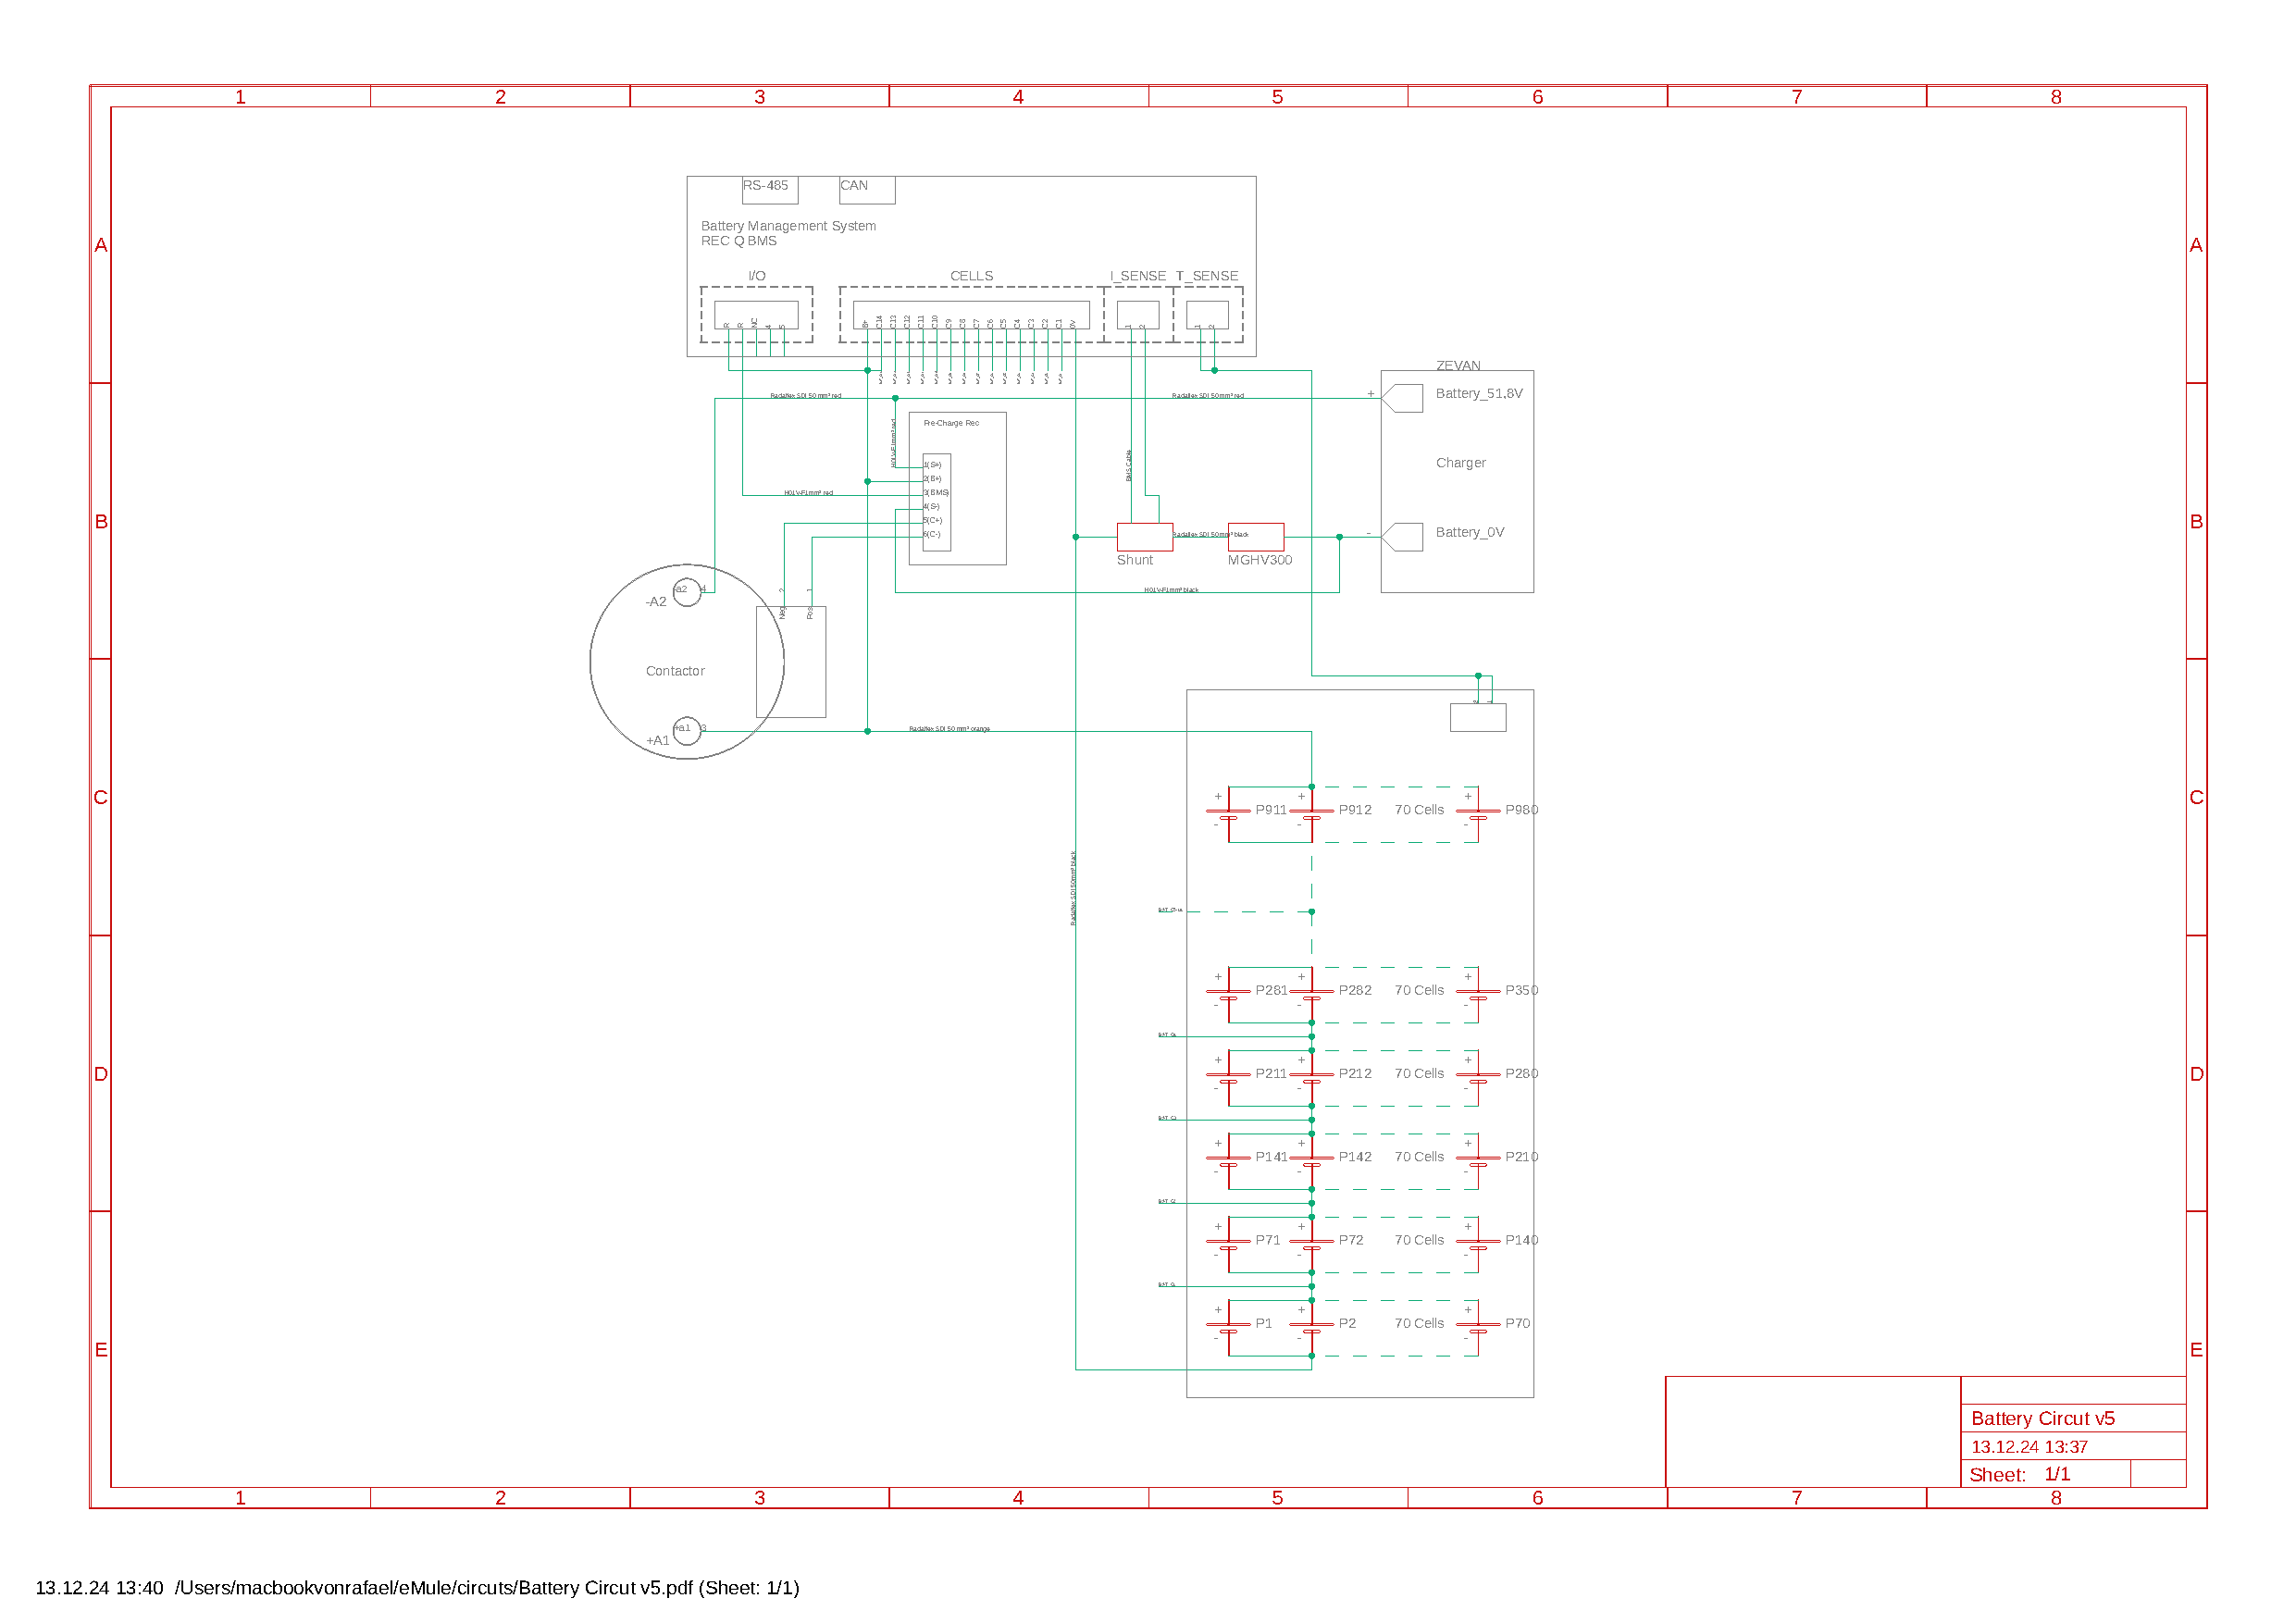
\includepdf[pages=1, fitpaper=true]{circuts/Battery Circut v5.pdf} 
\addtocounter{page}{1} 
\section*{Schaltplan Motor Controller v7}
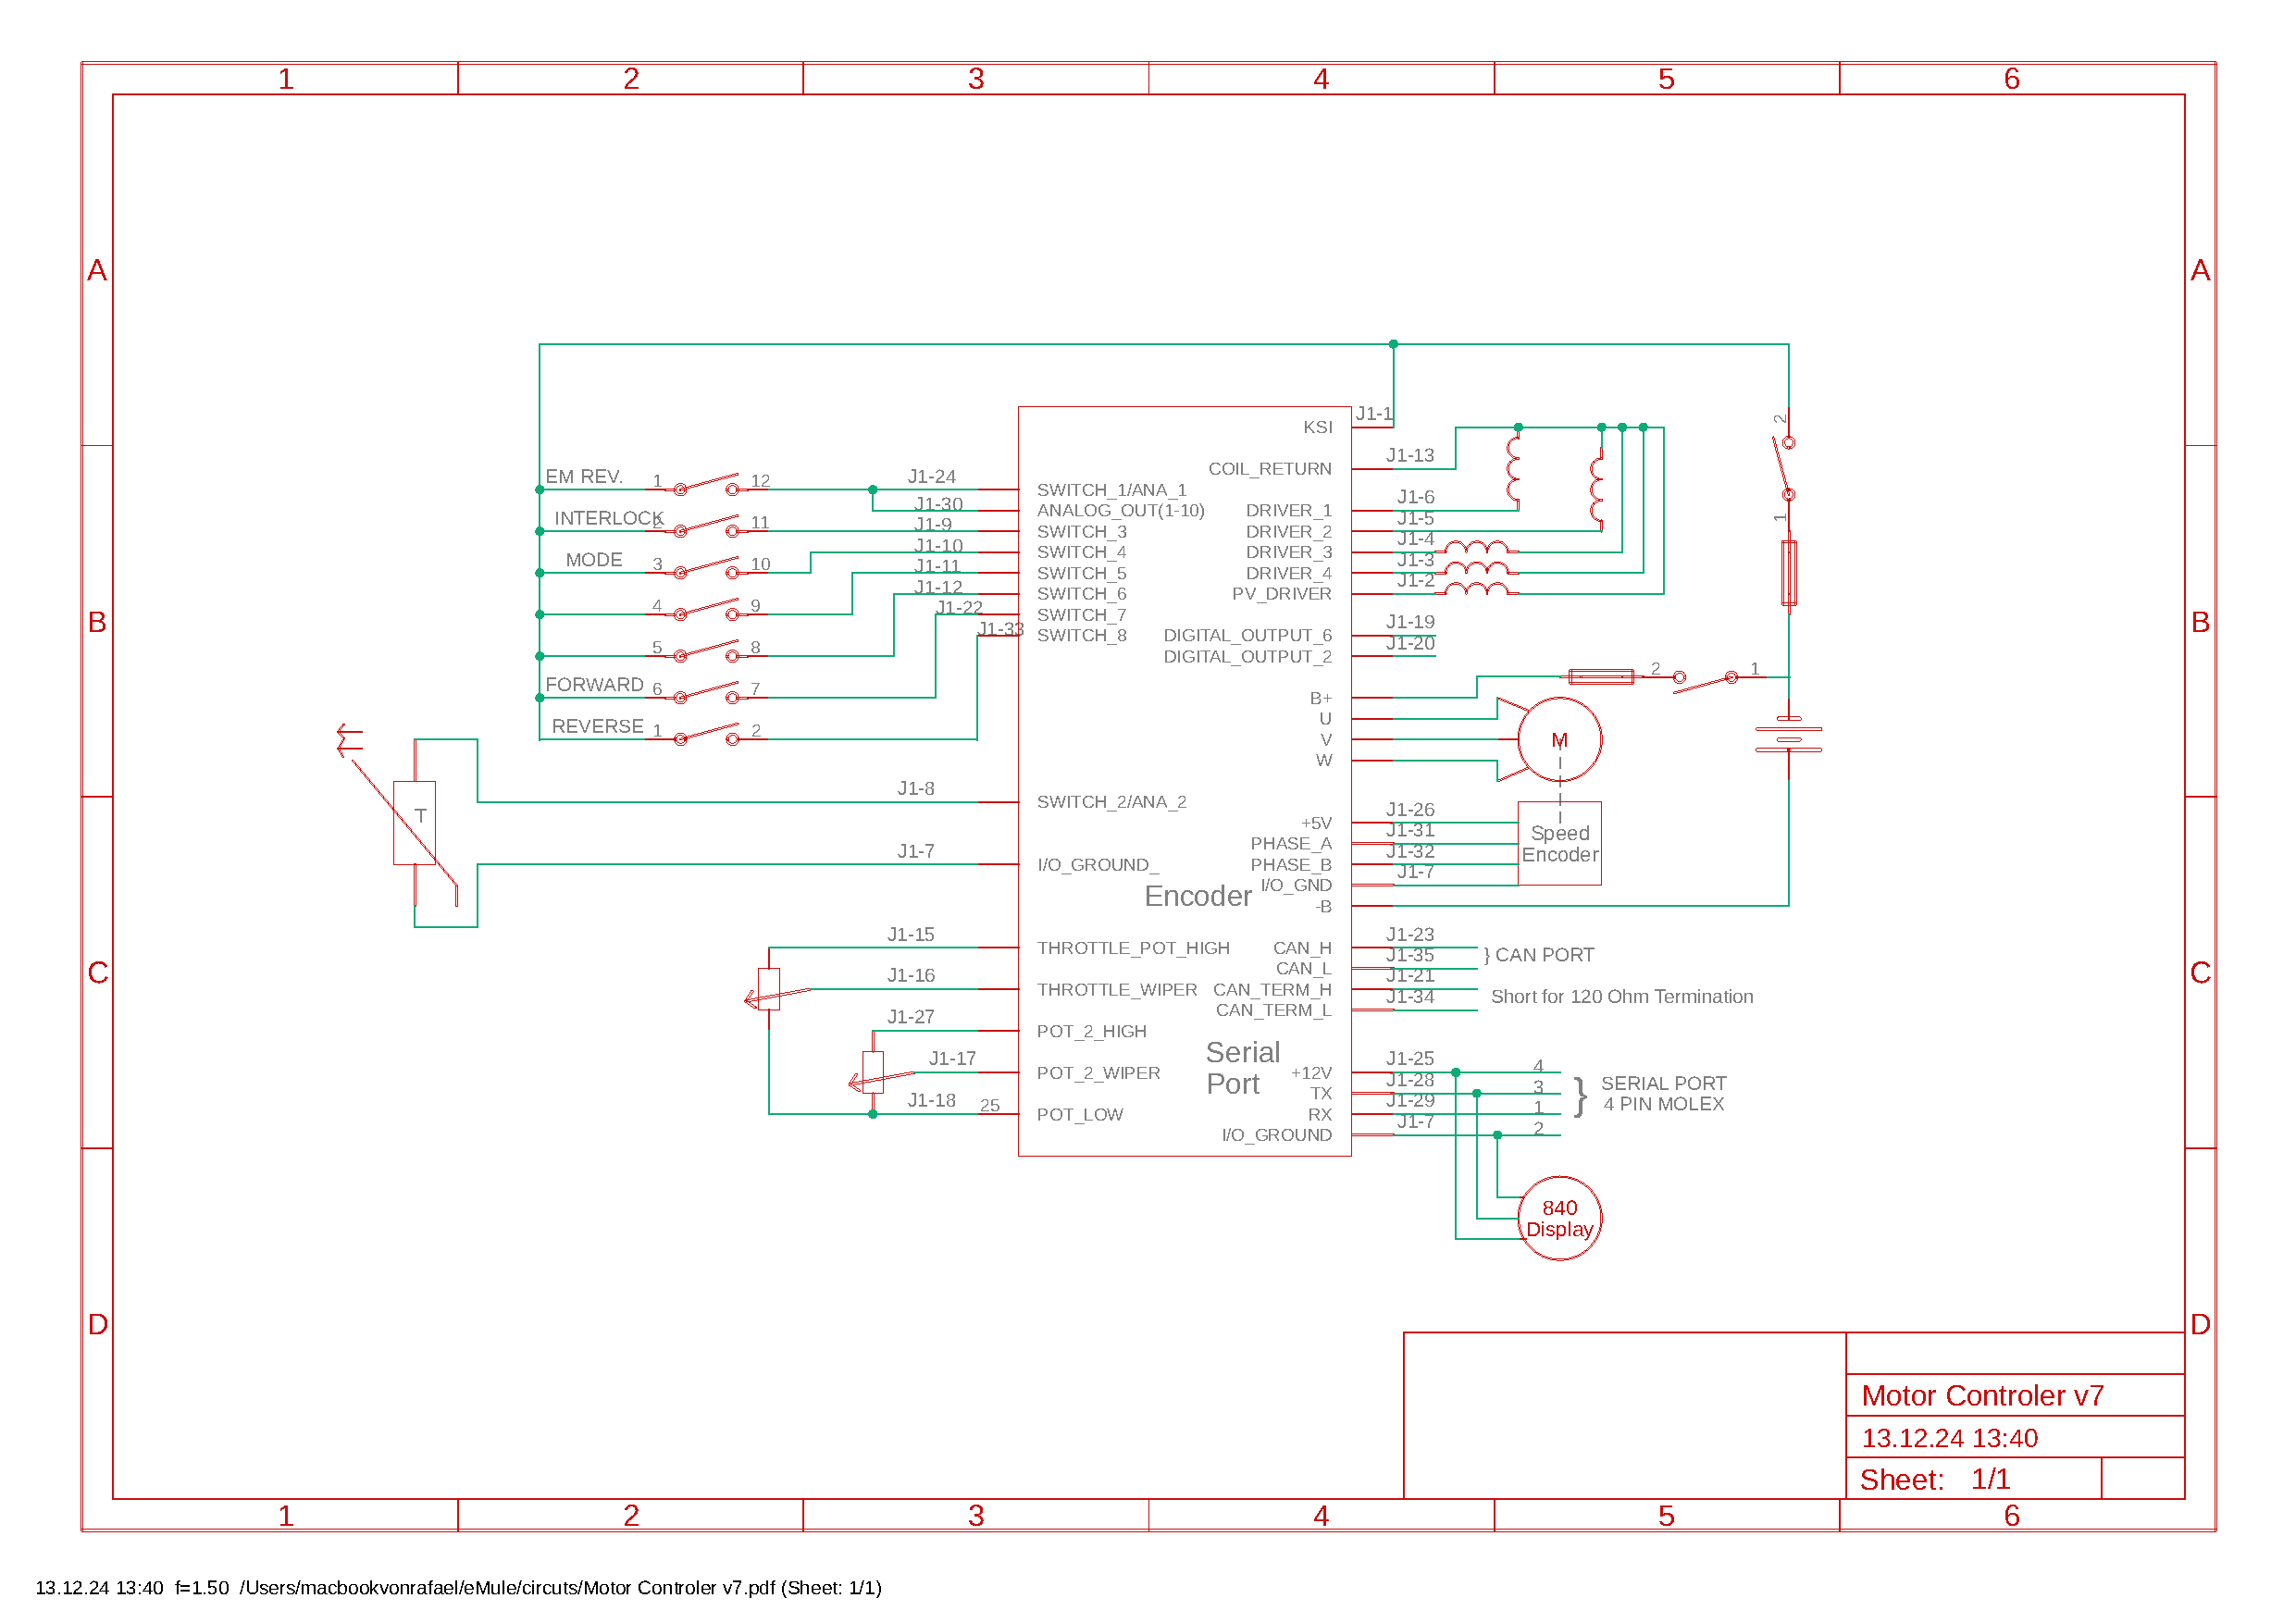
\includepdf[pages=1, fitpaper=true]{circuts/Motor Controler v7.pdf} 
\addtocounter{page}{1} 
\section*{Schaltplan Onboard-Netz v14}
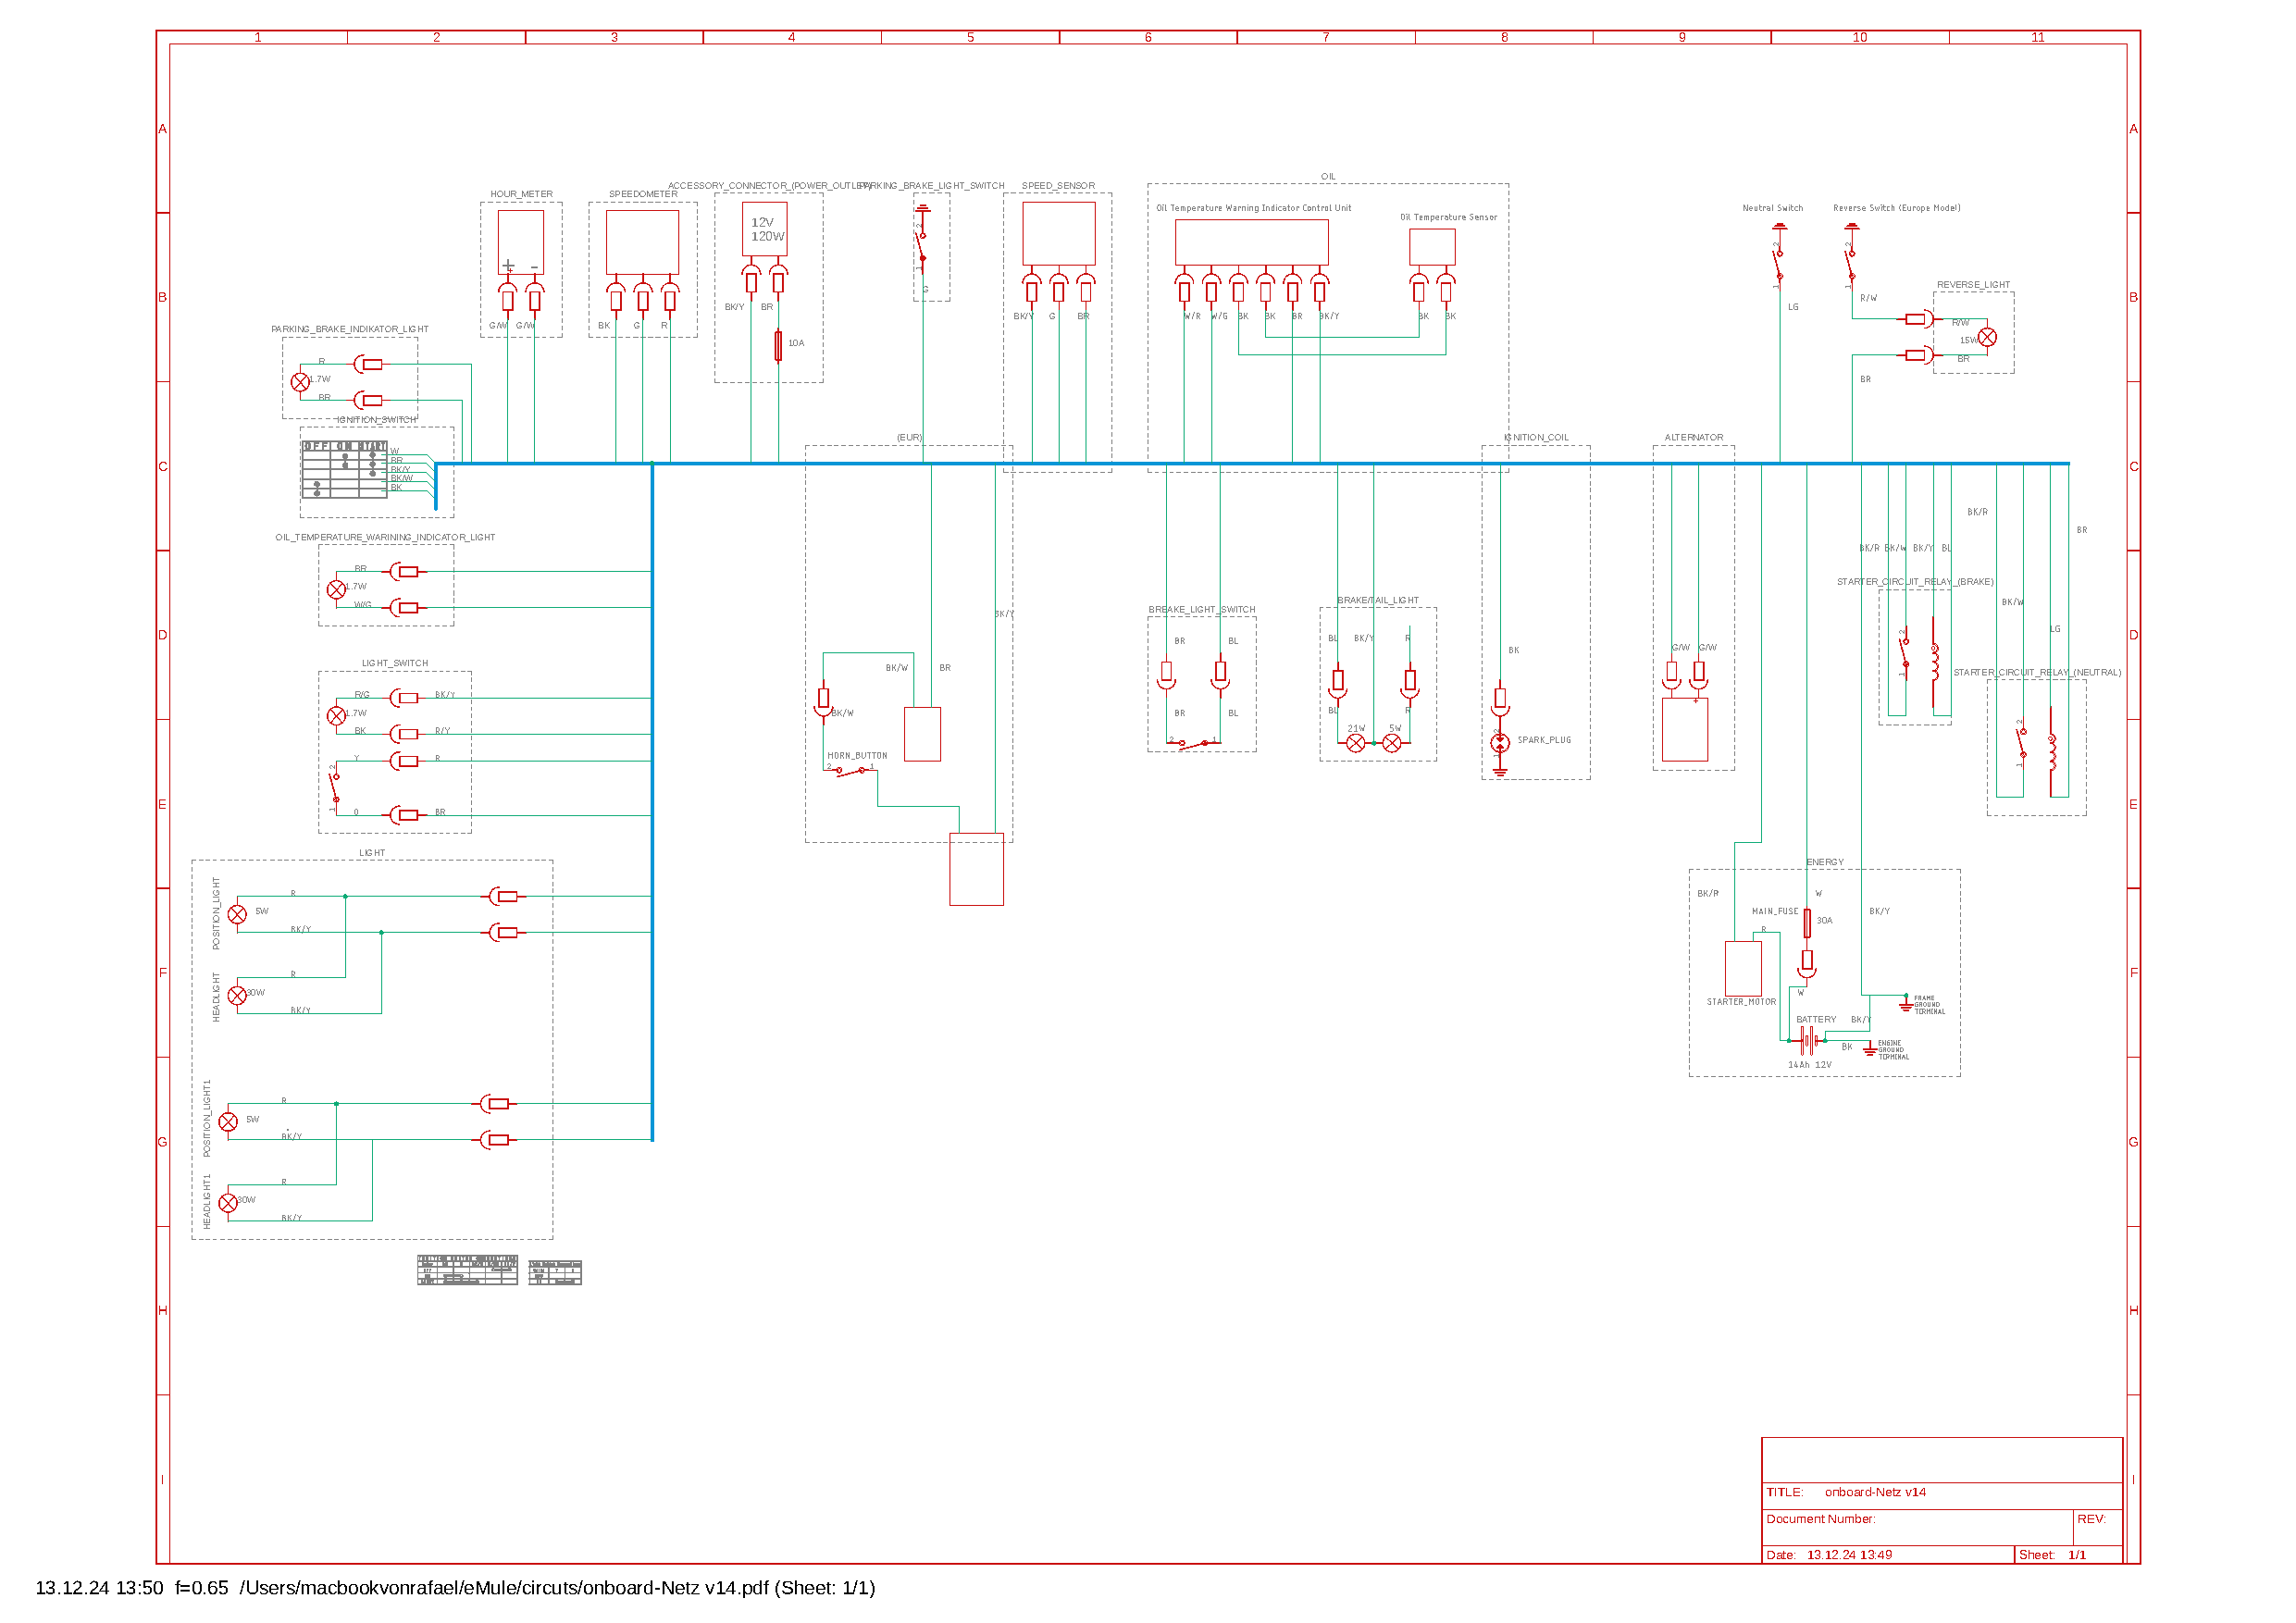
\includepdf[pages=1, fitpaper=true]{circuts/onboard-Netz v14.pdf} 
\addtocounter{page}{1} 
\section*{Temperatursteuerung des Ladegeräts v7}
\includepdf[pages=1, fitpaper=true]{circuts/Temperatursteuerung des Ladegerätes v7.pdf} 
\addtocounter{page}{1} 